\documentclass[a4paper, USenglish, cleveref, autoref, thm-restate]{lipics-v2021}

\usepackage{hyperref}
\bibliographystyle{plainurl}

\title{Formally verifying a vertical cell decomposition algorithm}

\author{Yves Bertot}{Inria Center at Université Côte d'Azur, France}
       {yves.bertot@inria.fr}
       {https://orcid.org/0000-0001-5052-3019}{}

\author{Thomas Portet}{Inria Center at Université Côte d'Azur, France}
       {thomas.portet@inria.fr}
       {}{}


\authorrunning{Y. Bertot and T. Portet}

\Copyright{Yves Berto and Thomas Portett}


\ccsdesc[300]{Theory of computation~Computational geometry}
\ccsdesc[500]{Theory of computation~Program verification}
\ccsdesc[500]{Theory of computation~Higher order logic}
\ccsdesc[500]{Theory of computation~Logic and verification}
\ccsdesc[500]{Theory of computation~Type theory}

\keywords{Formal Verification, Motion planning, algorithmic geometry}



%Editor-only macros:: begin (do not touch as author)%%%%%%%%%%%%%%%%%%%%%%%%%%%%%%%%%%
\EventEditors{John Q. Open and Joan R. Access}
\EventNoEds{2}
\EventLongTitle{42nd Conference on Very Important Topics (CVIT 2016)}
\EventShortTitle{CVIT 2016}
\EventAcronym{CVIT}
\EventYear{2016}
\EventDate{December 24--27, 2016}
\EventLocation{Little Whinging, United Kingdom}
\EventLogo{}
\SeriesVolume{42}
\ArticleNo{23}
%%%%%%%%%%%%%%%%%%%%%%%%%%%%%%%%%%%%%%%%%%%%%%%%%%%%%%

\begin{document}
\maketitle

\begin{abstract}
We design a succession of algorithms to decompose a finite area of the
plane into cells in such a way that none of these cells contain obstacles.
We provide a formally verified proof that this produces safe cells,
obtained using the Rocq prover and the mathematical components library.

This article discusses the assumptions made concerning the area and the
obstacles the structure of the main algorithm, especially the way it handles
the possibility of degenerate cases, the specification of the final safety
property, the organisation of the formal proof.
\end{abstract}

\section{Introduction}
The formal verification of algorithms is often presented as a solution
to avoid programmation errors.  It is particularly suited to domains
where it is practical to give a mathematical description of the
problem and expected behaviors and where the cost of errors is
prohibitive.

In recent years, there has been much progress in the design and
acceptance of autonomous vehicles.
In the long run, we wish to describe formally 
software that plans trajectories
for complex objects.  One of the first case studies that comes to mind
is concerned with proving that a program producing trajectories for a
point in a bi-dimensional scene is safe.  We designed such a program,
and its first component is concerned with reading the description of
the scene and constructing a decomposition into cells, where each cell
helps describing where it is safe to evolve.

We chose to study an algorithm described in the book {\em Robot Motion
  Planning} by J.-C. Latombe under the name ``vertical cell
decomposition''.  In that book's presentation, the obstacles are
described as polygons, but we chose to simplify the problem by
considering only obstacles described using straight line segments.
Our algorithm is a simple generalization, since any polygon can be
decomposed in a collection of edges corresponding to the polygon's
boundary.

This algorithm is sweeping line algorithm.  It can be described
intuitively as the process of moving a line from left to right over
the scene, stopping each time an event is encountered.
Events occur when the extremities of obstacles are encountered.
Several obstacles may be concerned by a single event: Several
obstacles that were present on the left side the sweeping line may be
finishing at this event, and several obstacles may be starting at this
event.

When processing an event, the algorithm produces two kinds of cells.
Some of the new cells are {\em open}.  They are in a temporary state,
where only the left-hand side is known, actually this side is aligned
with the sweeping line.  The other new cells are {\em closed}.  These
cells are obtained by collecting all the cells that are in contact
with the processed event and giving them a right side, again aligned
the current location of the sweeping line.

The lateral sides of each cell are vertical, because the sweeping line
is vertical.  Most of the points on these sides are safe, but
sometimes there is a point on one of these sides that is not safe,
because it is the location of an event, most often an extremity of an
obstacle.  The algorithm is designed in such a way that the unsafe
points on each lateral side are given with each closed cell.

For the use case that we have in mind, it is also important that cells
are non empty.  To guarantee this property, we had to design specific
tests and corrective actions when two successive events are vertically
aligned.  So instead of processing events from left to right, which is
not precise enough, we process events in lexical order: from left to
right if the successive events have a different first coordinate, and
from bottom to top for events that have the same first coordinate.

The algorithm is described entirely using the functional programming
language of the inductive calculus of constructions, as implemented in
Rocq.  The input is given as a bounding box and a list of obstacles.
The output is a list of cells.  There are quite a few expected
properties for the inputs: the obstacles should all be entirely inside
the bounding box and no obstacle should be vertical.  In return, we
obtain a list of cells that satisfy a few properties: the union of all
the cells are disjoint, each cell contains a safe part that is guaranteed to
have an empty intersection with the obstacles, and the safe part of
each cell is guaranteed to be non-empty.  All these properties have
been formally formally verified using the rocq prover and the {\sc
  Mathematical Components} library.

There is an extra property for which the proof has not be done yet:
the union of all cells and their boundaries covers the entire space in the
bounding box.

The complete development of the algorithm and its proof is available
in the following branch of a publicly available repository
\begin{center}
\url{https://github.com/math-comp/trajectories/tree/vertical-cells-paper}.
\end{center}
This branch contains the snapshot that is described in this paper, but
the whole development is likely to evolve as more improvements are
added to the algorithm and the use case resting on it, as discussed in the
last part of this paper.

\section{The data components}
In this section, we describe the design choices for the various kind
of data we manipulate in the algorithm.  The way we handle obstacles
deserves special attention.
\subsection{points and edges}

For the proofs, ww assume that we work with a type {\tt R} of numbers
with the structure of a real field, as understood by the
{\sc Mathematical Components} library.  Among other operations, this
mathematical structure provides a boolean test for equality between
numbers and boolean test for comparison.  The library then provides a
lot of tools with their properties, like a boolean test for list
membership, sorting, etc.  In practice, this means that
the field of rational numbers is suitable for all computations
performed in this development.

Points are then described as pairs of numbers in {\tt R}, and edges
are described as pairs of points.  These datatypes inherit the
equality tests and the polymorphic functions for list membership of
the {\sc Mathematical Components} library can again be used for these
datatypes.  One peculiarity of our development
is that we chose to describe the edges as pair of points with an extra
condition in our proofs: the first point has to have a first
coordinate that is strictly smaller than the right coordinate of the
second point.  This is an example of design where some data invariant
is hard-coded in the data structure.  As a result, the algorithm
cannot process vertical obstacles, because the data structure
representing the obstacles simply does not accept such cases.  In the
last part of the paper, we discuss ways to circumvent this limitation
concerning vertical edges.

The definition we use to introduce edges in our development is as
follows
\begin{verbatim}
Record edge := Bedge {left_pt : pt; right_pt : pt;
    _ : left_pt.x < right_pt.x}.
\end{verbatim}
This definition does not give a name to the condition that the left
point has a smaller first coordinate.  Such a name is given later in
our development.

The most important basic block used in the algorithm is the
computation of whether a point {\tt p} is above or under an edge, or whether
it is aligned with the two extremities of the edge.  To compute this
condition, it is well known in computational geometry \cite{Knuth} that the
following determinant can be used, where {\tt l} and {\tt r} are the
names for the left and right extremities of the edge:
\[\begin{array}{|ccc|}
1 & {\tt l}_x & {\tt l}_y\\
1 & {\tt r}_x & {\tt r}_y\\
1 & {\tt p}_x & {\tt p}_y\\
\end{array}\]
This is a determinant computation, and it is well known that this
determinant computes twice the {\em signed} area of the triangle {\tt
  lrp}.  The function {\tt area} computes this determinant.
Because it is a signed area, the value is positive if {\tt p}
is above and negative if {\tt p} is below.  We use the notations
{\tt \(p\) <<= \(g\)} {\tt \(p\) <<< \(g\)} to express that a point
\(p\) is in the half plane below an edge \(g\) or strictly below an
edge, respectively.

Because the algorithm uses a vertical sweeping line, our proofs
require that we check when a point is in the vertical cylinder
containing the edge.  This is simply done by comparing the point's
first coordinate with the first coordinates of the edge's extremities.
We write {\tt valid\_edge \(g\) \(p\)} to express that \(p\) is in
that cylinder.  We use the notation {\tt p === g} to express that
point {\tt p} is included in the obstacle (the {\tt area} function
returns 0 and {\tt valid\_edge} holds (the function is named
{\tt point\_on\_edge}.

When a point is valid for an edge, the vertical projection of that
point on that edge exists.  It is computed by a function called
{\tt vertical\_projection}.  Computing the vertical projection of a
point on an oblique edge requires that one computes a division.  This
is the one place in the whole algorithm where division is used.
The function {\tt vertical\_projection} takes a point and an edge as
arguments and returns an {\tt option} type:
the projection is only computed if the point is in the vertical
cylinder given by the edge.  We prove a few properties of this
projection function: the point it returns is part of the edge on which
the projection happens, two points with the same second coordinate are
projected to the same point, and the input point and its projection
are vertically aligned.

We define a relation between edges, noted {\tt <|} which expresses
that the first edge is below the second one.  Edge \(g_1\) is below Edge
\(g_2\) if both extremities of \(g_1\) are in the half plane below
\(g_2\) of if both extremities of \(g_2\) are in the half plane above
\(g_1\).  During the operation of the algorithm, we use this relation
to sort edges going out of a given event.  For edges that all have the
same left extremity, the {\tt <|} relation is transitive, but in
general this relation is not transitive.
\subsection{The cells}
Each cell has a high edge, a low edge, a left side, and the right side.  For
the lateral sides, we record the ordered sequence of points that
correspond  to events in contact with this cell.  These points are
unsafe.  These two sequences of points are called the {\em left
  points} and {\em right points} of the cell.  These sequences are
ordered and contain no duplication, so that the open interval between two
points in a sequence is a door, a safe passage to another cell.

The safe part of a cell is defined as the union of its strict interior
(points whose first coordinate is strictly between the left-side and
the right-side, strictly above the low edge, and strictly below the
high edge) and its doors (points on each of the sides that are
strictly abouve the low edge and strictly below the high edge and
different from the side points).

\begin{figure}
\includegraphics[trim={0 18cm 0 4cm}, clip,scale=0.5]{one_closed_cell.pdf}
\caption{A closed cell}
\end{figure}

Some cells have a side reduced to a single point, when the low edge
and the high edge meet.  We expect cells to have low edges and high
edges that meet at most one point, which must be an extremity for both
edges.  Moreover, the algorithm is designed in such a manner that the
left side of the cell is different from the right side.

In a finished closed cells, the sides are not empty, as they always
contain the projections of some event on the low and high edge, which
may be the same point.

As an intermediate data structure, we use cells where the
right-hand side is empty, called {\em open cells}  but in the code
there is never an ambiguity as to whether some cell is open or closed.

\section{The scan state}

The sweeping part of the algorithm is essentially a tail recursive
algorithm, consuming a sorted sequence events and
maintaining a datastructure which we call the {\tt scan\_state}.  This
structure contains a representation of the closed cells constructed so
far, a representation of all the open cells in contact with the
current position of the sweeping line, and some cached information:
the first coordinate of the last processed event, the high edge of the
last open cell.

The open cells are arranged in a vertically sorted sequence,
decomposed in three parts.  The middle part is a cell that is singled
out because it is the highest of the last created cells (in this
paper, we shall call this the {\em last open cell}.  The other two
parts are the prefix of the vertical sorted sequence before the last
open cell and the suffix of that sequence.

The closed cells are arranged in two parts, as the algorithm may need
to modify the last generated closed cell in some case.

\section{The phases of the algorithm}
To organize the sweeping process, we work in two phases.
\begin{enumerate}
\item  We first
create a sorted sequence of events.  Processing this sequence of
events actually implements the sweeping movement from left to right.
\item Process each event in turn, removing it from the sequence of
  events, and modifying only the scan state.
\end{enumerate}

An event is the pair of a point and a sequence of edges, with the
intended data-invariant
that all edges in the sequence have that point as their left
extremities.  In contrast with what was done for edges, we chose not
to encode this intended invariant in the data structure, so that it
would be possible to build events where the sequence of edges do not
satisfy this property.  This never happens in the algorithm, and there
is a formal proof of this fact.

To create the sequence of events,
We use a bespoke insertion-sort algorithm, where the insertion
procedure is designed to create new events only when no event with the
same point already exist in the sequence.  When adding edges to an
event, we do not produce a sorted sequence of edges.  Such a sorting
operation of the outgoing sequence of edges is performed later in the
algorithm.

When processing each event four cases are treated differently:
\begin{itemize}
\item If the considered event is further right than the last processed event
\item If the considered event is on the same vertical line, but above the
high edge of the last created open cell
\item If the considered event is on the same vertical line, but below the
high edge of the last created open cell
\item If the considered event is on the high edge of the last created open cell
\end{itemize}

To obtain the initial scan state, we need to have already one closed
cell, which is only constructed after the first event is processed.
This first closed cell has the left side of the bounding box as left
side, and its right side contains exactly three points: the first
event, its projection on high boundary of the bounding-box, and its
projection on the low boundary of the bounding-box.  The first
sequence of open cells is obtained by constructing new open cells
using the sorted sequence of outgoing edges from the first event.  If
the sequence of events is directly the one obtained after sorting a
set of edges, then the first event will have outgoing edges, but the
sweeping algorithm is also designed to accept events that have no
incoming and no outgoing edges.  When the first event has at least
one outgoing edge, the initial last open cell is a cell whose low edge
is the highest outgoing edge and whose high edge is the bounding box
high boundary, with only two points in the left point sequence: the
projection of the event on the high boundary and the event itself.
When the first event has no outgoing edge, the initial last open cell
has the bounding box low boundary as low edge and the bounding box
high boundary as high edge, its sequence of left points contains the
event and the two projections on the boundaries.
\begin{figure}
\includegraphics[trim={0 23cm 0 0}, clip,scale=0.5]{initial_state.pdf}
\caption{Two possible configurations for the initial scan state}
\end{figure}

\subsection{Work performed in the first case}
When the next event to be processed is not vertically aligned with the
previous one, we need to scan the current sequence of open cells to
know which of these cells will be affected by the current event.
These cell simply are the cells for which the current event is below
the high edge and above the low edge.  We call these cells the {\em
  contact cells}.  These cells are a sub-sequence
of the current sequence of open cells.  The function that computes
this sequence actually returns several meaninful pieces of data:
\begin{enumerate}
\item the prefix of unaffected cells,
\item the sequence of contact cells without the last one,
\item the last contact cell,
\item the suffix of unaffected cells
\item the low edge of the first contact cell,
\item the high edge of the last contact cell
\end{enumerate}
The function that computes that decomposition is called
{\tt open\_cells\_decomposition}.  It takes as input a point and a
sequence of cells.  We proved that under some assumptions, the
sequence of cells given as input is the concatenation of the prefix,
the contact cells, and the suffix, and that the two edges given as
output are indeed boundary edges of the first and last contact cells.

All contact cells are transformed into closed cell, by adding a
right-side.  When there is more that one contact cell, the first one
has as low edge an edge that is not in contact with the current event
and as high edge an edge whose right point is the current event.
Similarly, the last contact cell has as high edge an edge that is not
in contact with the current event as low edge an edge whose right
point is the current event.  So, when there is more than one contact
cell, the first and the last are created with a sequence of right
points containing two points: the current event and the projection of
that event on another edge to which it does not belong.

When there is only one contact cell, this is because the processed
event is below that cell's high edge and above that cell's low edge.
The sequence of the right points for the new cell only contains three
points, the event and its projections to the cells two edges.

All contact cells are removed from the list of open cells, but new
open cells, whose left side contains the currently processed event are
added in their place.  The new open cells are obtained by processing
recursively the sequence of outgoing edges, sorted with respect to the 
{\tt <|} relation (also known as {\tt edge\_below}).

\subsection{Work performed for the second case}
In the second case, we know that the last open cell is not among the
contact cells.  We call the function {\tt open\_cell\_decomposition},
but we only need to scan the suffix of the sequence of open cells (the
cells that are above the last open cell).  The rest of processing is
the same as in the first case, paying attention to the fact that the
prefix and the previous last open cell have to be included in the
resulting sequence of open cells.

\subsection{Work performed for the third case}
In the third case, the event is below the high edge of the last open
cell, and this even cannot be the right extremity of
an active edge, because there is no edge between the low and the high
edge of the last open cell.  For this reason, it is not necessary to
re-run the {\tt open\_cells\_decomposition} function, as it would
simply return the last open cell as the last contact cell, and no
other contact cell.  Closing this contact cell to produce a new closed
cell is not suitable, because it would create an empty closed cell
(one where the first coordinate would be the same on both lateral
sides).

No new closed cell is created, but the last closed cell needs to be
updated because the current event is an extra unsafe point that needs
to be added to its sequence of right points.  This requirement
explains why the scan state has a specific field for the last closed cell.

New open cells need to be created.  If the current event has no
outgoing edges, then it is enough to update the last open cell by adding
the current event among its unsafe points on the left side.  If the
current event has outgoing edges, new open cells are created as in the
first two cases, but the sequence of unsafe points that were present
in the last open cell needs to be included in the sequence of left
points of the first newly created open cell.
\begin{figure}
\begin{center}
\includegraphics[trim={0 0 0 0}, clip,scale=0.5]{third_case.pdf}
\end{center}
\caption{Processing a degenerate case: the processed event appears on
  the last open cell left boundary and on the last closed cell right
  boundary.  The unsafe points that were previously in the last open
  cell left point sequence need to be added to the first newly created
  open cell (here noted as {\sf new open cell \# 1}.
  }
\end{figure}

\subsection{Work performed for the fourth case}
In the fourth case, the processed event is on the high edge of the
last open cell.  We know that the last open will be the first of
contact cells, and we need to compute the other contact cells, by
calling {\tt open\_cells\_decomposition}, but this time with a sequence
of cells that starts with the last open cell.

When closing cells, the first contact cell does not need to be closed
and can simply discarded, because all the unsafe points were already
taken into account by existing closed cells, and the current event was
already a member of the right point sequence for the last closed cell
(because it is equal to the projection on the last closed cell high
edge of the previous event).

When creating new open cells, special attention is required for the
case where the event has no outgoing edges.  In this case, the last
open cell needs to be replace with an open cell that has as low edge
the same low edge as the the last open cell, as high edge the high
edge of the last contact cell
(as computed by {\tt open\_cells\_decomposition}) and as sequence of
last points the sequence of left points from the last open cell where
the projection on the high edge has been added.

\subsection{Specifying the behavior}
This paper describes a proof of safety, there are desirable properties
that will not be subject to a formal proof.  The safety property will
be expressed in the following manner: any point in the safe part of a
closed cell is distinct from the obstacles and the events given as
input.  We already defined the safe part of closed cells in the
section about cells.

In a similar manner, we can describe unsafe locations as points lying
on an obstacle, as described by the function {\tt point\_on\_edge}.

We prove that the intersection between unsafe locations and the union
of all safe parts of the resulting closed cells is empty.

However, we have to be careful because this proof is done under a
collection of assumptions.
\begin{itemize}
\item The type of numbers provided to describe the point coordinates,
  the edges, alignment of points, and so on, with its operation and
  comparison predicates form an ordered field structure.
\item The only allowed intersections between obstacles are at their
  extremities.
\item The sequence of obstacles does not contain any duplications.
\item all obstacle extremities are inside the
bounding box.
\end{itemize}
When propagating this specification to the two phases, it turns out we
need the following specification for the sorting phase.
\begin{enumerate}
\item The union of all outgoing edges of all events in the sorted
  sequence of events contains the initial obstacles.
\item For a given event, all outgoing edges have the same left
  extremity, located at this event.
\item The sequence of events is strictly sorted alphabetically.
\item No event in the sequence appears in the middle of one of the
  obstacles.
\item The right extremity of every outgoing edge is also located at an
  event existing in the sequence of events.
\item All events are inside the bounding box.
\end{enumerate}
With respect to the safety property, this means that we can consider
variants of the algorithm where more events are added in the sequence,
as long as these properties are respected.  In particular,
We plan to add isolated events for points that are not in contact with
any obstacles.

If the sequence of events is produced from an initial sequence of
obstacles, then events are always extremities of obstacles.  However,
the second part of the program, which processes the sequence of events
does not make the assumption that events are always on edges.  It can
actually process events that describe isolated points that do not
belong to any obstacle (neither extremities nor points in the middle
of the segment).  When specifying the safety
property for the results of the algorithm, we simply need to make sure
that these orphaned events are not part of the safe subset of the
configuration space.

A property that does not appear immediately as a safety property is
that the middle of every cell is strictly included in the cell.  This
property is useful for users of this algorithm who wish to use a cell
as turning space to move from one door of the cell to another door of
the same cell, when both doors are on the same side.  This property is
the main reason for having a specific treatment for degenerate cases.
This specific treatment actually guarantees that every closed cell has
a left-hand side with an x-coordinate that is lower than the
x-coordinate of the right-hand side.

To make sure that every cell contains at least a safe point, we
actually need the property that every event has a list of outgoing
edges without duplications.  Our code to generate the sequence of
events does not include steps to guarantee this, but if the input
list of obstacles has no duplications, the code does not duplicate them.

\section{Proving the safety property}
\subsection{Mirroring contexts}
The infra-structure of definitions provided by the Mathematical
Components library is not fully compatible with the extraction
process.  To obtain code that is amenable for extraction, we write a
first file called {\tt generic\_trajectories}, that does not rely on
any of the mathematical structures present in math comp, but is
parameterized by a given type supposed to represent numbers, with 4
operations (addition, subtraction, multiplication, division) and two
comparisons.  Also, this algorithm relies on a degraded type of edges,
where the condition that the first point is on the left of the second
point is absent from the data-structure.

The generic algorithm is used in all the proof files.  In each of
these proof files, we open a section where the type of numbers is
actually provided by a structure of type {\tt realFieldType}.  It
should be noted that all the proofs performed about this algorithm
only rely on the fact that the type of numbers forms a field, so that
any implementation of rational numbers is for making all the
computations.

Every function imported from {\tt generic\_trajectories} is a function
with at least 7 arguments.  To make the whole setup comfortable, a
header of notation definition is provided to instantiate the function
to the type and operations provided by the field structure.


\subsection{Main organization of the proof}
The first part of the algorithm consists in preparing the list of
events, processing these events in the order given by the list
simulates the intuitive behavior of moving a vertical line
progressively from the left-hand side of the box to the right-hand
side.

The algorithm maintains a sequence of open cells between two events,
the topological properties of these cells are preserved as one moves
from one event to the next: the low and high edges of the cell are the
same, the neighbor cells on the other side of these edges are the
same, etc.  Only when an event occurs does the structure of the list
of open cells change.  Some cells that were present in the list of
open cells are removed from that list, and after some modification,
they are added to the list of closed cells, new cells are created
where the low or high edge, or both, are taken from the outgoing edges
of the currently processed event.

This feels like reasoning by homotopy.  Depending on the position of
the sweeping line, the intersections between these lines and the low
and high edges of each open cell are at different heights, but these
points are always ordered on this line in the same manner.  In other
words, the topological structure of the sequence of cells evolves
continuously as the sweeping line moves from one event to the other.
This relies on a strong invariant concerning the sequence of events:
any change of topology (for example the end of an active edge) must be
recorded in the sequence of events.  This is reflected by two
predicates {\tt close\_alive\_edges} and {\tt close\_edges\_from\_events}.

In our work, we rely quite a lot on a relation between edges, named
{\em edge\_below} and noted by the infix symbol {\tt <|}.  It turns
out that this relation is reflexive, not transitive, and not
antisymmetric, so many of the tools we
would like to inherit from the ambient formal mathematics library
cannot be used directly out of the box.

In the proof, we established five levels of invariants:
\begin{enumerate}
\item In the first level, we state properties that concern only the
sequence placement of low and high edges for the open cells,
\item In the second level, we add the cache consistency properties of
  the scan state, the expected properties of the sequence of events,
  and the consistency between the open cells and the future events,
\item In the third level, we add properties that are specific to the
  last created cell,
\item In the third level, we add mainly the properties that concern
  the closed cells that were built so far and their interactions with
  the current open cells.  The main purpose of the properties
  available in this invariant is to contribute to the proof that
  all closed cells are disjoint and non-empty.
\item In the fourth level, we add mainly the properties that concern
  processed edges and their coverage by existing closed and open
  cells.
\item In the fiftth level, we add mainly the properties that concern
  the points recorded in cell sides.  The point is to show that cell
  sides enumerate the points that are unsafe on the vertical
  sides of cells.
\end{enumerate}
In the end, the safety property for the space inside a given cell was
guaranteed by the main argument that if edges are covered by the high
edges of all closed cells, and all closed cells are disjoint, then
edges cannot appear in the interior of a given cell.

We performed two proofs of the main result.  The first proof takes
stronger assumptions on the inputs: it assumes that two events are
never vertically aligned.  If this is the case, no specific treatement
is needed to handle the last created open cell, which is guaranteed to
be transformed later into a non-empty closed cell.  The second proof
observes the case where verical alignment of events is permitted.  In
this case, it sometimes necessary to not create new open cells, but
only to modify existing cells.n
\subsection{Algebraic properties of the area function}
The area function is instrumental to detect when a point is above or
below an edge.  More precisely, it makes it possible to detect when a
point is above the straight line that carries the obstacle.

This area function is given by a determinant formula that we learned
from Knuth, but is probably part of the folklore in algorithmic
geometry.  It is quite important that this is only computed using a
determinant, as it only needs ring operations (no division), without
ever mentioning the projection of the given point on the given
straight line.

For proofs, however it is useful to have an alternative point of view,
where one expresses the property of being above using a comparison of
the second coordinates of the given point with the projected point on
the given line.

The edge comparison relation is directly related with the area
function.  To detect whether an edge is below another, we simply
verify whether the two extremities of one are in the same half plane
with respect to the other.

In the end, to express that a point lies on a segment, we use the area
function to detect that the point is aligned with the extremities, and
using the invariant that no obstacle is given is vertical, we simply
verify that the first coordinate is between the first coordinates of
the segment extremities.
\subsection{Building up invariants}
\subsection{The key property of disjoint cells}
In the end, each closed cell has four boundaries: two vertical ones, a
low boundary (a fragment of an obstacle that is not vertical) and a
high boundary (again, not vertical).  We define three zones:
\begin{itemize}
\item inside the union of the cell and its boundaries,
\item strictly inside the cell, not on the boundaries,
\item inside the cell and its
 boundaries, but neither on the bottom boundary nor on the left
 boundary.  In the rest of the paper, we say a point that satisfies
 this property with respect to a cell is {\em attached to the cell}.
 We say that two cells are disjoint if no point can be attached to
 both of them.
\end{itemize}
The main key property that we want to guarantee is that every point
strictly inside a cell does not belong to any obstacle.  To establish
this, we decompose the problem in two parts: first we show
that points can only be attached to one cell.  Later, we
prove that every obstacle is included the union of high boundaries of
all cells, this makes it possible to conclude with the key property.

To prove that closed cells are disjoint, we need to prove that new
cells added at each iteration are disjoint with the existing ones.
The new closed closed cell actually come from
existing open cells.  Therefore, we need to prove the invariant that
closed cells are disjoint from open cells, and in turn, we need to
show that open cell are disjoint.

The position of the sweeping line plays an important role when proving
that existing closed cells and open cells are disjoint.  At any
iteration, the newly created cells have their left side on the
sweeping line.  On the other hand, newly closed cells have their right
side on the sweeping line.  Moreover, since the sweeping line is moving
from left to right, all previously existing closed cells have their
right side on the left of the sweeping line.

In the degenerate case where two successive events are vertically
aligned and the second event lies below the high edge of the last
closed cell created when processing the first event, this last closed
cell is modified and the new modified cell becomes the last closed
cell after processing the second event.  We need to guarantee that
the modification does interfere with the disjointness property with
respect to the other cells.  This is given to us by the fact that the
points attached to last closed are the same before and after the
modification (which consists only in adding the second event to
sequence of right points in the cell, in second position).  Because
our model of the algorithm follows the style of functional
programming, the modified cell is logically a completely different cell,
and we need to be very explicit about the fact that the modified cell
is disjoint with any other cell because the un-modified cell already
was.

\marginpar{\textcolor{blue}{not sure about this par, probably useful,
    but not the right place.}}
Just expressing that the two cells have the same attached point is not
logically sufficient, because the two cells could have an empty set of
attached points.  It turns out that our algorithm only produces
non-empty cells, so we chose to add to our collection of invariant
properties the fact that any closed cell contains at least one point:
the cell center, computed by as first coordinate the middle between
the left and right sides, and as second coordinate, the middle of the
intersections between the low and high boundaries of the cells.
\subsection{Obstacle covering}
As the sweep line progresses from left to right, more and more events
are processed, and the obstacles whose leftmost point is at the
processed event are included in the boundaries of existing cell.  The
property that is invariant here, is that every obstacle belonging in
the outgoing edges from an event that has already been processed is
included in the high boundaries of a collection of cells, with two
important cases:
\begin{itemize}
\item If the event corresponding to the right extremity of the
  obstacle is yet to be processed, then the rightmost part of the
  obstacle is included in the high boundary of an open cell,
\item Otherwise, the obstacle is completely included in the high
  boundaries of a collection of adjacent closed cells.
\end{itemize}

When an event is processed, the cell decomposition algorithm computes
a sequence contact cell together with a last contact cell.  The latter
is meant to become the future last closed cell.  It high edge is the
same obstacle as the high edge of future last open cell.  If we
are in general position (the current event is not vertically aligned
with the previous one) This high
edge was covered by the combination of a sequence of closed cells and
an open cell before this iteration, and after this iteration, the
sequence of closed cells receives a new element (the last contact cell
that was just closed) and the new last open cell still participates in
its covering.

For the high edges of all the other contact cells, they are
necessarily ending in the current event.  So these obstacles move from
the category of obstacles that are partially covered by open cells to
the category of obstacles that completely covered by closed cells.

If we are in the degenerate position where the current event is
vertically aligned with the previous event and below the high edge of
last closed cell, then the sequence of closed cells that participate
in covering this edge keeps the same number of elements: the previous last
closed cell is removed and replaced by the the modified closed cell
where the event is added among its right points.  The portion of the
obstacle that is covered by the previous last closed cell and the
modified cell is the same.  Concerning coverage by an open cell, the
new last open cell has the same high edge as the previous one, and
they have the same left side, because the two events that created
these open cells are vertically aligned.
\subsection{Safety for points strictly inside cells}
In the end, there are no more events left to process, so that all
obstacles are covered by closed cells.  
We can guarantee that points strictly inside these closed cells are not
on obstacles by combining the edge covering property and the
dijointness property.  If we name \(c_1\) a closed cell and \(p\) an
point inside that cell, then \(p\) cannot be on the high edge of
\(c_1\) by definition of ``strictly inside''.  If \(p\) is on an
obstacle, this obstacle is covered by cells, so that there must be a
cell \(c_2\) such that \(c_2\) contains \(p\) and \(p\) is on the high
edge of \(c_2\).  Because \(p\) is not on the high edge of \(c_1\),
\(c_1\) and \(c_2\) must be distinct, but by the definition of
attached points, \(p\) must be attached to both \(c_1\) and \(c_2\).
\subsection{Safety for points on the lateral boundaries}
For each closed cell, our algorithm provides two sequences of points
corresponding to the points on the left and right boundary that are
unsafe.  We need to prove that the other points are safe, so that they
can be used to compute trajectories that move from on cell to a
neighboring one.

One of the key way to prove that all cells have a safe left side is to
observe the following facts:
\begin{itemize}
\item After an event is processed, all cells that are likely to
  contain this event have this event as an element of their left point
  sequences,
\item If a point appears in the left point sequence of an open cell
  that is not the last open cell, an iteration either preserves that
  open cell, or creates a closed cell with the same sequence of left
  points,
\item In degenerate cases where the last open cell is modified to
  produce a new last open cell, the sequence of left points for the
  new last open cell contains the previous sequence of left points to
  which the currently processed event is being added.
\end{itemize}

Proving that all cells have a safe right side follows a similar track:
\begin{itemize}
\item Apart from the last closed cell, we know that no closed cell is
  in contact with the currently processed event,
\item All newly created closed cells when processing an event have
  that event inside their right point sequence,
\item In degenerate cases where the last closed cell is modified to
  produce a new last closed cell, the sequence of right points for new
  last closed cell contains the previous sequence of right points to
  which the currently processed event is being added.
\item In degenerate cases where the processed event is on the high
  edge of the last closed cell, the last closed cell is transfered
  directly to the regular closed cells, and the processed event is
  already in the sequence of right points of the cell, because it is
  the projection of the previous event on the high edge of the cell.
\end{itemize}
\section{Conclusion}
\subsection{A basis for trajectory computation}
Because we only prove safety, the specification studied in this paper
could be fulfilled by a stupid program that returns an empty sequence
of cells.  As a way to assess usability, we actually developed an
application that uses this vertical cell decomposition algorithmm to
produce a trajectories between points in the configuration space, when
such a trajectory exists.

It is possible that no trajectory exists between two points in the
safe part of the configuration space, because obstacles could be used
to delimit polygons, and no trajectory exists between the interior and
the exterior of a polygon.  

To compute trajectories between points that are not in the same cell,
we need to recognize when two cells are neighbors with a safe passage
between them.  For now, we compute this neighboring relation by
computing for each cell what are the intervals between successive
points in the left points or the right points of that cell.  This
gives us doors out of that cell.  Two cells are neighbors with a safe
passage if they have a door in common.  Cells, together with the
neighboring relation, constitute a graph in which with can perform a
discrete search for a path between cells.  
To compute a trajectory, we
thus only have to find the cells that containing the source and target
of that trajectory, then find a path between these cells, then
transform this path into a path between doors.

When the trajectory needs to go from one door into a cell to a door in
the other side of the cell, a straight line can be used between a
point in the first door and the second door.  On the other hand, when
a trajectory needs to go from one door into a cell to another door on
the same side, a straight line cannot be used, because this would
collide with extremities of both doors.  For this case, we need to
build a path that goes from the first door strictly inside the cell,
and then to the second door.  This is why we made the effort to have
an algorithm that only produces non-empty cells: we have the guarantee
that a point inside the cell always exists for this kind of need.
\subsection{Vertical obstacles in trajectory computation}
\subsection{Concerning numerical computation}
When considering safety of trajectory computation, we need to
anticipate the problems that may arise because of the fact that
computers do not implement the idealized computations that are
envisioned in the formal model.

It should be noted that the computation performed in the area function
is just second-degree multivariate polynomial.  These computations can
be made exact at a little cost, taking into account the discretization
that necessarily happens when perceiving the environment.  A robot may
be designed to work with sensors that yield coordinates in 16 bits.
When this happens, the computations performed in the area function
will be exact if they are performed with a processor computing with 32
bits (a rough estimate).

However, there is a part of the algorithm that performs a division,
this is when computing the projection of a point on an edge.  This
point is stored in the result of the cell decomposition as an extremal
point in the sequence of left points or the sequence of right points
of closed cell.  It is later used when computing trajectories.  One
important feature of this computation is that {\em it is not used to
  take decisions during the vertical cell decomposition}.  It is just
data that is stored for later usage.

Since this value is not needed right away, we could decide not to
compute it, but to store it as the intersection between a vertical
line (whose position is given as input) and an obstacle (whose
extremities are given as input).  The consumer algorithm, in our case
the algorithm responsible to compute trajectories can then decide
whether the exact value is required, or whether an approximation
suffices.  To compute trajectories, these intersection points appear
higher or lower extremities of safe doors, and they can safely be
replace by points with a lower approximation or a higher approximation
of the second coordinate, respectively.

As future work, we wish to refine the algorithm so that it produces
cells where the sequences of left points and right points are not in
the datatype of pairs of coordinates, but rather in a sum type, where
a point is given either as a pair of coordinate or the pair of a first
coordinate and a obstacle in which we take the point with that first
coordinate, so that the information is processed in the right away by
the following algorithms.
\subsection{Concerning the neighboring relation}
In our use case to compute trajectories, we need to know what are the
neighbors of each closed cell.  It seems obvious that this information
is already known at the time an open cell is created and could be
propagated along as the cells are added in the final cell of closed
cells.  If we refine the algorithm so that this information is
constructed and preserved, the result of the algorithm will not be a
sequence of closed cells, but a graph whose nodes are closed cells and
edges are the doors between cells.  The safety property would be the
same as the one that we have already proved: the safe part of each
cell must have no intersection with the obstacles.  The correctness of
the graph would stand as follows: if there is an edge between two
nodes, then the corresponding door is included in the safe part of the
cells it connects.

To make this proof easier, we need a way to keep track of the life of
closed cells as they are created.  It turns out that a bit of
imperative programming could help here.  When closed cells are
created, we store them in a sequence, but this sequence could be
viewed as an array, so that closed cell stored in that array never
moves afterwards, and the index in that array can be used as a unique
identifier for that cell.  Special care must be taken concerning cells
that are modified after their creation, like the last closed cell.
\subsection{Concerning obstacle crossing}
This vertical cell decomposition algorithm works under a strong
assumption that the edges describing the obstacles do not cross.  This
assumption deserves a discussion.

Given a pair of straight line segments that have an intersection, it
is rather easy to compute that intersection and then decompose the two
segments into two, three, or four segments that only intersect at
their extremities and cover the same subset of the plane.  The
intersecting obstacles can then be replaced by the new segments and
the precondition of the algorithm is satisfied.

A first approach that can be implemented and
proved is to process the initial list of segments, compute all pairs
of two obstacles, and for each of these pairs detect whether this
decomposition must be performed.  It is annoying that this process
will have a quadratic cost in the number of obstacles that need to be
processed.

A second approach that can be implemented is to integrate the
treatment of crossing obstacles directly in the vertical cell
decomposition algorithm.  In fact, after each iteration, it is only
necessary to check whether two neighboring high edges of open cells
intersect, peform the needed replacement and add the intersection as a
new event to be treated later.  It is interesting to understand
whether the current research concerning algorithm refinement could
help proving this improved algorithm with optimal reuse of the proofs
that were already performed for the naive algorithm.  We plan to study
such a refinement as future work.

However, an algorithm that replaces pairs of crossing segments by
segments that touch only at their extremities has the default that it
relies on division (in the case where four new segments are produced,
one needs division to determine the coordinates of
the intersection point).  When factoring in our concern for
approximations in numeric computations, it becomes necessary to understand how
rounding errors in this division process will affect the operation of
the algorithm.  We may choose to replace the exact point with an
approximation, assuming that the obstacles defined with this
approximation as extremity as close enough to the original obstacles
for the results to be safe.  We may even be able to quantify the risk
of collision induced by this kind of replacement.

In practice, it may be perfectly acceptable to live with the
constraint that obstacles do not cross.  It depends on the source of
the scene description.  If the scene description was drawned by a
human being using a computer aided design tool, then intersections are
likely.  If the scene is the result of a process involving sensors and
post-processing, it is possible that the post-processor already
guarantees that the scene description is given by polygons whose edges
do not intersect.
\end{document}
